\vspace*{-17mm}
\begin{activite}[Des petits cubes]
    \begin{changemargin}{-5mm}{-10mm}
    {\bf Objectifs :} déterminer le volume d'un solide par dénombrement ; analyser un solide en trois dimensions.
       \partie[des cubes de cubes]
          Donner le nombre de petits cubes qui composent chacun des solides suivants : \\
          \begin{center}
            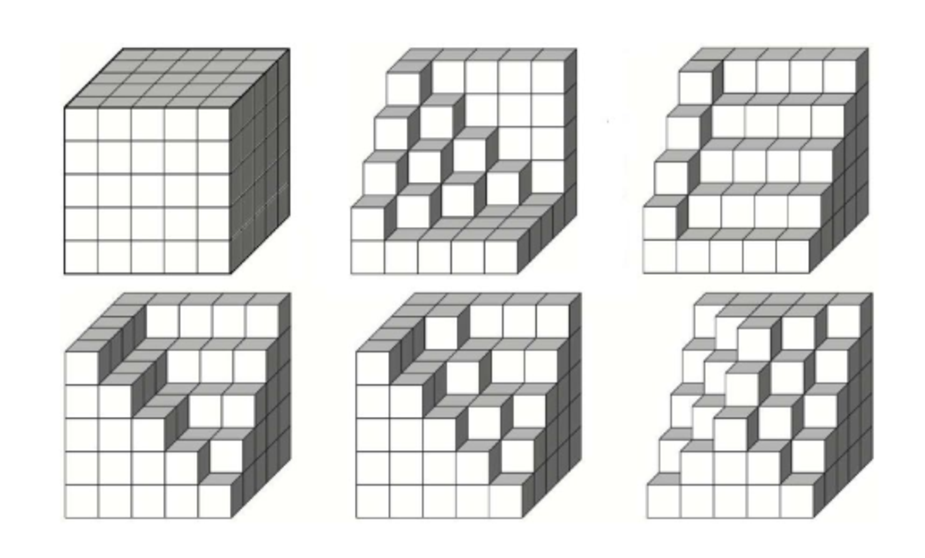
\includegraphics[width=15cm]{\currentpath/images/cube}
          \end{center}          
       \partie[à vous de jouer !]
          Dessiner trois solides différents comportant huit petits cubes chacun.
          \begin{center}
             {\psset{unit=0.5}
             \begin{pspicture}(0,-0.5)(30,10.5)
                \psgrid[subgriddiv=1,gridlabels=0,gridcolor=lightgray](0,0)(30,10)
                \psframe(1,7)(2,8)
                \pspolygon[fillstyle=solid,fillcolor=lightgray](1,8)(1.5,8.5)(2.5,8.5)(2,8)
                \pspolygon[fillstyle=solid,fillcolor=gray](2.5,8.5)(2,8)(2,7)(2.5,7.5)
             \end{pspicture}}
          \end{center}
        \vfill\hfill{\it\footnotesize Source : \href{http://www-irem.univ-paris13.fr/site_spip/spip.php?article348}{IREM Paris-Nord}}
        \end{changemargin}
 \end{activite}
 